\section{Executing COMPSs applications}
\label{sec:Executing}


\subsection{Prerequisites}
\label{subsec:prerequisites}
Prerequisites vary depending on the application's code language: for Java applications the users need to have
a \textbf{jar archive} containing all the application classes, for Python applications there are no requirements and for
C/C++ applications the code must have been previously compiled by using the \textit{buildapp} command.

For further information about how to develop COMPSs applications please refer to the \textit{COMPSs User 
Manual: Application development guide} available at the \url{http://compss.bsc.es/} webpage.


\subsection{Runcompss command}
\label{subsec:runcompss}
COMPSs applications are executed using the \textbf{runcompss} command:
\begin{lstlisting}[language=bash]
compss@bsc:~$ runcompss [options] application_name [application_arguments]
\end{lstlisting}

The application name must be the fully qualified name of the application in Java, the path to the \textit{.py} file
containing the main program in Python and the path to the master binary in C/C++. 

The application arguments are the ones passed as command line to main application. This parameter can be empty. 

The \textit{runcompss} command allows the users to customize a COMPSs execution by specifying different options.
For clarity purposes, parameters are grouped in \textit{Runtime configuration}, \textit{Tools enablers}
and \textit{Advanced options}.

\begin{lstlisting}[language=bash]
compss@bsc:~$ runcompss -h

* Options:
  General:
    --help, -h                              Print this help message

    --opts                                  Show available options

    --version, -v                           Print COMPSs version
    
  Tools enablers:
    --graph=<bool>, --graph, -g             Generation of the complete graph (true/false)
                                            When no value is provided it is set to true
                                            Default: false
                                            
    --tracing=<level>, --tracing, -t        Set generation of traces and/or tracing level
                                            ( [ true | basic ] | advanced | false)
                                            True and basic levels will produce the same traces.
                                            When no value is provided it is set to true
                                            Default: false
                                            
    --monitoring=<int>, --monitoring, -m    Period between monitoring samples (milliseconds)
                                            When no value is provided it is set to 2000
                                            Default: 0
                                            
    --external_debugger=<int>,
    --external_debugger                     Enables external debugger connection on the 
                                            specified port (or 9999 if empty)
                                            Default: false

  Runtime configuration options:
    --task_execution=<compss|storage>       Task execution under COMPSs or Storage.
                                            Default: compss
                                            
    --storage_conf=<path>                   Path to the storage configuration file
                                            Default: None
                                            
    --project=<path>                        Path to the project XML file
                                            Default: /opt/COMPSs/Runtime/configuration/
                                            xml/projects/default_project.xml
                                            
    --resources=<path>                      Path to the resources XML file
                                            Default: /opt/COMPSs/Runtime/configuration/
                                            xml/resources/default_resources.xml  
                                            
    --lang=<name>                           Language of the application (java/c/python)
                                            Default: java
                                            
    --log_level=<level>, --debug, -d        Set the debug level: off | info | debug
                                            Default: off

  Advanced options:
    --comm=<path>                           Class that implements the adaptor for communications
                                            Supported adaptors: 
                                             integratedtoolkit.nio.master.NIOAdaptor
                                             | integratedtoolkit.gat.master.GATAdaptor
                                            Default: integratedtoolkit.nio.master.NIOAdaptor
                                            
    --scheduler=<path>                      Class that implements the Scheduler for COMPSs
                                            Supported schedulers: 
                                             integratedtoolkit.components.impl.TaskScheduler 
                                             | integratedtoolkit.scheduler.readyscheduler.ReadyScheduler
                                            Default: integratedtoolkit.scheduler.readyscheduler.ReadyScheduler
                                            
    --library_path=<path>                   Non-standard directories to search for libraries 
                                            (e.g. Java JVM library, Python library, 
                                            C binding library)
                                            Default: Working Directory
                                            
    --classpath=<path>                      Path for the application classes / modules
                                            Default: Working Directory
                                            
    --base_log_dir=<path>                   Base directory to store COMPSs log files 
                                            (a .COMPSs/ folder will be created inside this location)
                                            Default: User home
                                            
    --specific_log_dir=<path>               Use a specific directory to store COMPSs log files 
                                            (the folder MUST exist and no sandbox is created)
                                            Warning: Overwrites --base_log_dir option
                                            Default: Disabled
                                            
    --uuid=<int>                            Preset an application UUID
                                            Default: Automatic random generation
                                            
    --master_port=<int>                     Port to run the COMPSs master communications.
                                            Only for NIO adaptor
                                            Default: 43000
                                            
    --jvm_master_opts="<string>"            Extra options for the COMPSs Master JVM. 
                                            Each option separed by "," and without 
                                            blank spaces (Notice the quotes)
                                            Default: 
                                            
    --jvm_workers_opts="<string>"           Extra options for the COMPSs Workers JVMs.
                                            Each option separed by "," and without 
                                            blank spaces (Notice the quotes)
                                            Default: -Xms1024m,-Xmx1024m,-Xmn400m
                                            
    --task_count=<int>                      Only for C/Python Bindings. Maximum number 
                                            of different functions/methods, invoked from 
                                            the application, that have been selected as tasks
                                            Default: 50
                                            
    --pythonpath=<path>                     Additional folders or paths to add to the PYTHONPATH
                                            Default: /home/cramonco/svn/compss/framework/trunk/compss
                                            
    --PyObject_serialize=<bool>             Only for Python Binding. Enable the object 
                                            serialization to string when possible 
                                            (true/false).
                                            Default: false


* Application name:
    For Java applications:   Fully qualified name of the application
    For C applications:      Path to the master binary
    For Python applications: Path to the .py file containing the main program

* Application arguments:
    Command line arguments to pass to the application. Can be empty.

\end{lstlisting}

\subsection{Running a COMPSs application}
\label{subsec:running_compss}
Before running COMPSs applications the application files \textbf{must} be in the \textbf{CLASSPATH}.
Thus, when launching a COMPSs application, users can manually pre-set the \textbf{CLASSPATH} environment variable
or can add the \textit{--classpath} option to the \textit{runcompss} command.

The next three sections provide specific information for launching COMPSs applications developed in different code languages (Java, Python and 
C/C++). For clarity purposes we will use the \textit{Simple} application (developed in Java, Python and C++) available in the COMPSs
Virtual Machine or at \url{https://compss.bsc.es/projects/bar} webpage. This application takes an integer as input
parameter and increases it by one unit using a task. For further details about the codes please refer to the \textit{Sample 
Applications} document available at \url{http://compss.bsc.es} .

\subsubsection{Running Java applications}
A Java COMPSs application can be launched through the following command:
\begin{lstlisting}[language=bash]
compss@bsc:~$ cd workspace_java/simple/jar/
compss@bsc:~/workspace_java/simple/jar$ runcompss simple.Simple <initial_number>
\end{lstlisting}

\begin{figure}[h!]
  \centering
    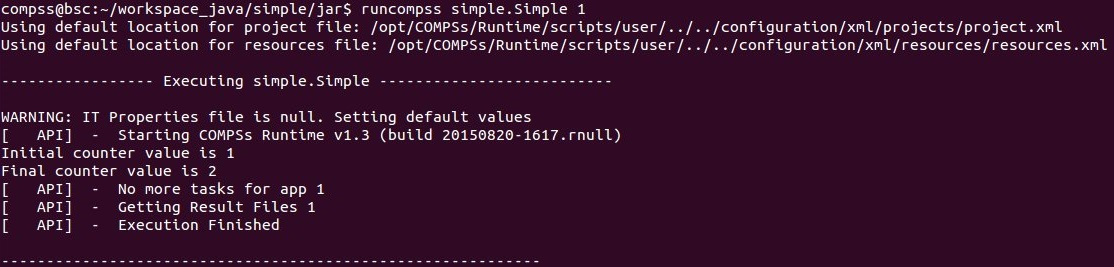
\includegraphics[width=\textwidth]{./Sections/2_Execution/Figures/java_execution.jpeg}
    \caption{Execution of a Java COMPSs application.}
    \label{fig:java_execution}
\end{figure}
\vspace{-0.4cm}

In this first execution we use the default value of the \textit{--classpath} option to automatically add the jar
file to the classpath (by executing runcompss in the directory which contains the jar file). However,
we can explicitly do this by exporting the \textbf{CLASSPATH} variable or by providing the 
--classpath value. Next, we provide two more ways to perform the same execution:

\begin{lstlisting}[language=bash]
compss@bsc:~$ export CLASSPATH=$CLASSPATH:
                               /home/compss/workspace_java/simple/jar/simple.jar
compss@bsc:~$ runcompss simple.Simple <initial_number>
\end{lstlisting}

\begin{lstlisting}[language=bash]
compss@bsc:~$ runcompss --classpath=/home/compss/workspace_java/simple/jar/simple.jar 
                        simple.Simple <initial_number>
\end{lstlisting}


\subsubsection{Running Python applications}
To launch a COMPSs Python application users have to provide the \textit{--lang=python} option to the runcompss command. 

\begin{lstlisting}[language=bash]
compss@bsc:~$ cd workspace_python/simple/
compss@bsc:~/workspace_python/simple$ runcompss --lang=python simple.py <initial_number>
\end{lstlisting}

\begin{figure}[h!]
  \centering
    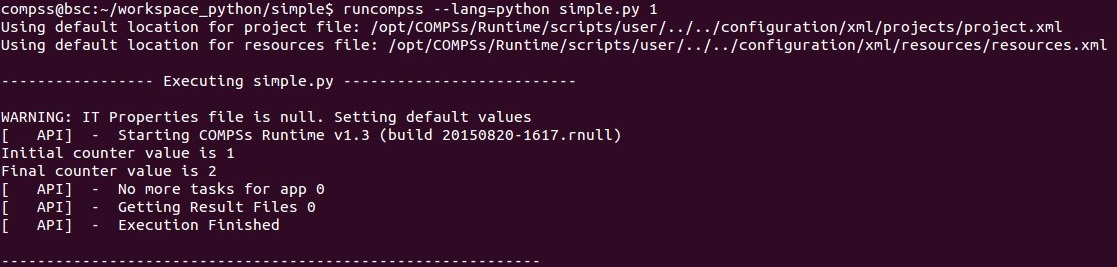
\includegraphics[width=\textwidth]{./Sections/2_Execution/Figures/python_execution.jpeg}
    \caption{Execution of a Python COMPSs application.}
    \label{fig:python_execution}
\end{figure}
\vspace{-0.4cm}


\subsubsection{Running C/C++ applications}
To launch a COMPSs C/C++ application users have to compile the C/C++ application by means of the \textit{buildapp} command. For 
further information please refer to the \textit{COMPSs User Manual: Application development guide} document available at \url{http://compss.bsc.es} . Once complied, 
the \textit{--lang=c} option must be provided to the runcompss command.

\begin{lstlisting}[language=bash]
compss@bsc:~$ cd workspace_c/simple/
compss@bsc:~/workspace_c/simple$ runcompss --lang=c simple <initial_number>
\end{lstlisting}

\begin{figure}[h!]
  \centering
    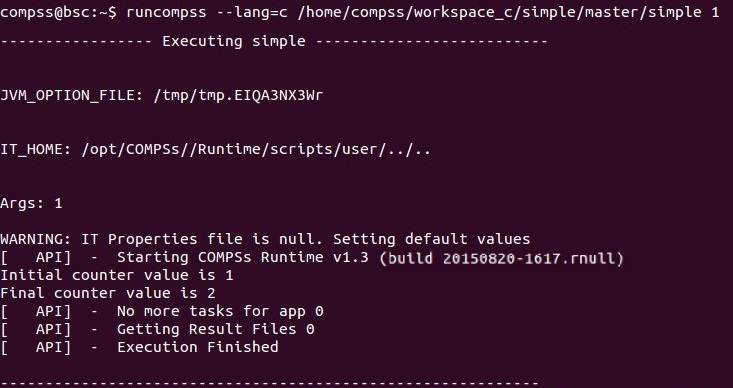
\includegraphics[width=0.95\textwidth]{./Sections/2_Execution/Figures/c_execution.jpeg}
    \caption{Execution of a C++ COMPSs application.}
    \label{fig:c_execution}
\end{figure}
\vspace{-0.4cm}


\subsection{Additional configurations}

The COMPSs runtime has two configuration files: \textit{resources.xml} and \textit{project.xml} . 
These files contain information about the execution environment and are completely independent from the application.

For each execution users can load the default configuration files or specify their custom configurations 
by using, respectively, the \textit{$--resources=<absolute\_path\_to\_resources.xml>$} and the
\textit{$--project=<absolute\_path\_to\_project.xml>$} in the \textit{runcompss} command. The default files are located 
in the \emph{/opt/COMPSs/Runtime/configuration/xml/} path. 
Users can manually edit these files or can use the \textit{Eclipse IDE} tool developed for COMPSs. For further 
information about the \textit{Eclipse IDE} please refer to Section \ref{subsec:IDE}. 


Next sections describe in detail the \textit{resources.xml} and the \textit{project.xml} files, 
explaining the available options.

\subsubsection{Resources file}
The \textit{resources} file provides information about all the available resources that can be used for an execution. 
This file should normally be managed by the system administrators. Its full definition schema can be found at \\
\emph{/opt/COMPSs/Runtime/configuration/xml/resources/$resource\_schema$.xsd}. 

For the sake of clarity, users can also check the SVG schema located at \\
\emph{/opt/COMPSs/Runtime/configuration/xml/resources/$resource\_schema$.svg}.

This file contains one entry per available resource defining its name and its capabilities. Administrators can define several
resource capabilities (see example in the next listing) but we would like to underline the importance of 
\textbf{ComputingUnits}. This capability represents the number of available cores in the described resource and it is
used to schedule the correct number of tasks. Thus, it becomes essential to define it accordingly to the number of cores 
in the physical resource. 

\begin{lstlisting}[language=xml]
compss@bsc:~$ cat /opt/COMPSs/Runtime/configuration/xml/resources/default_resources.xml
<?xml version="1.0" encoding="UTF-8" standalone="yes"?>
<ResourcesList>
    <ComputeNode Name="localhost">
        <Processor Name="P1">
            %*{\bf $<ComputingUnits>4</ComputingUnits>$ }*)
            <Architecture>amd64</Architecture>
            <Speed>3.0</Speed>
        </Processor>
        <Processor Name="P2">
             %*{\bf $<ComputingUnits>2</ComputingUnits>$ }*)
        </Processor>
        <Adaptors>
            <Adaptor Name="integratedtoolkit.nio.master.NIOAdaptor">
                <SubmissionSystem>
                    <Interactive/>
                </SubmissionSystem>
                <Ports>
                    <MinPort>43001</MinPort>
                    <MaxPort>43002</MaxPort>
                </Ports>
            </Adaptor>
        </Adaptors>
        <Memory>
            <Size>16</Size>
        </Memory>
        <Storage>
            <Size>200.0</Size>
        </Storage>
        <OperatingSystem>
            <Type>Linux</Type>
            <Distribution>OpenSUSE</Distribution>
        </OperatingSystem>
        <Software>
            <Application>Java</Application>
            <Application>Python</Application>
        </Software>
    </ComputeNode>
</ResourcesList>
\end{lstlisting}


\subsubsection{Project file}
The project file provides information about the resources used in a specific execution. Consequently, the resources that 
appear in this file are a subset of the resources described in the \textit{resources.xml} file. This file, that contains
one entry per worker, is usually edited by the users and changes from execution to execution. Its full definition 
schema can be found at\\ 
\emph{/opt/COMPSs/Runtime/configuration/xml/projects/$project\_schema$.xsd}.

For the sake of clarity, users can also check the SVG schema located at \\
\emph{/opt/COMPSs/Runtime/configuration/xml/projects/$project\_schema$.xsd}.

We emphasize the importance of correctly defining the following entries:
\begin{description}
 \item [installDir] Indicates the path of the COMPSs installation \textbf{inside the resource} (not necessarily the same 
 than in the local machine).
 \item [User] Indicates the username used to connect via ssh to the resource. This user \textbf{must} have passwordless access to the
 resource (for more information check the \textit{COMPSs Installation Manual} available at our website \url{http://compss.bsc.es}).
 If left empty COMPSs will automatically try to access the resource with the \textbf{same username than the one that lauches 
 the COMPSs main application}.
 \item [LimitOfTasks] The maximum number of tasks that can be simultaneously scheduled to a resource. Considering that a task 
 can use more than one core of a node, this value must be lower or equal to the number of available cores in the resource. 
\end{description}


\begin{lstlisting}[language=xml]
compss@bsc:~$ cat /opt/COMPSs/Runtime/configuration/xml/projects/default_project.xml
<?xml version="1.0" encoding="UTF-8" standalone="yes"?>
<Project>
    <!-- Description for Master Node --> 
    <MasterNode\>

    <!--Description for a physical node-->
    <ComputeNode Name="localhost">
        %*{\bf $<InstallDir>/opt/COMPSs/</InstallDir>$ }*)
        <WorkingDir>/tmp/Worker/</WorkingDir>
        <Application>
            <AppDir>/home/user/apps/</AppDir>
            <LibraryPath>/usr/lib/</LibraryPath>
            <Classpath>/home/user/apps/jar/example.jar</Classpath>
            <Pythonpath>/home/user/apps/</Pythonpath>
        </Application>
        %*{\bf $<LimitOfTasks>4</LimitOfTasks>$ }*)
        <Adaptors>
            <Adaptor Name="integratedtoolkit.nio.master.NIOAdaptor">
                <SubmissionSystem>
                    <Interactive/>
                </SubmissionSystem>
                <Ports>
                    <MinPort>43001</MinPort>
                    <MaxPort>43002</MaxPort>
                </Ports>
                %*{\bf $<User>user</User>$ }*)
            </Adaptor>
        </Adaptors>
    </ComputeNode>
</Project>
\end{lstlisting}
\label{lstlisting:project.xml}


\subsection{Configuration examples}
In the next subsections we provide specific information about the services, shared disks, cluster and cloud configurations and several \textit{project.xml} and \textit{resources.xml} examples. 


\subsubsection{Services configuration}
To allow COMPSs applications to use WebServices as tasks, the \textit{resources.xml} can include a special type of resource called 
\textit{Service}. For each WebService it is necessary to specify its wsdl, its name, its namespace and
its port. 
\begin{lstlisting}[language=xml]
<?xml version="1.0" encoding="UTF-8" standalone="yes"?>
<ResourcesList>
    <ComputeNode Name="localhost">
      ...                                                                                                                                                                                                
    </ComputeNode>  
    
    <Service wsdl="http://bscgrid05.bsc.es:20390/hmmerobj/hmmerobj?wsdl">                                                                                                                                          
        <Name>HmmerObjects</Name>                                                                                                                                                                                  
        <Namespace>http://hmmerobj.worker</Namespace>                                                                                                                                                              
        <Port>HmmerObjectsPort</Port>                                                                                                                                                                              
    </Service>                                                                                                                                                                                                     
</ResourcesList>  
\end{lstlisting}

When configuring the \textit{project.xml} file it is necessary to include the service as a worker by adding an
special entry indicating only the name and the limit of tasks as shown in the following example:
\begin{lstlisting}[language=xml]
<?xml version="1.0" encoding="UTF-8" standalone="yes"?>                                                                                                                                                            
<Project>                                                                                                                                                                                                          
    <MasterNode/>                                                                                                                                                                                                  
    <ComputeNode Name="localhost">                                                                                                                                                                                 
      ...                                                                                                                                                                           
    </ComputeNode>   
    
    <Service wsdl="http://bscgrid05.bsc.es:20390/hmmerobj/hmmerobj?wsdl">                                                                                                                                          
        <LimitOfTasks>2</LimitOfTasks>                                                                                                                                                                             
    </Service>                                                                                                                                                                                                     
</Project> 
\end{lstlisting}

\subsubsection{Cluster and grid configuration (static resources)}
In order to use external resources to execute the applications, the following steps have to be followed:

\begin{enumerate}
 \item Install the \textit{COMPSs Worker} package (or the full \textit{COMPSs Framework} package) on all the new 
 resources following the \textit{Installation manual} available at \url{http://compss.bsc.es} .
 \item Set SSH passwordless access to the rest of the remote resources.
 \item Create the \textit{WorkingDir} directory in the resource (remember this path because it is needed 
 for the \textit{project.xml} configuration).
 \item Manually deploy the application on each node.
\end{enumerate}

The \textit{resources.xml} and the \textit{project.xml} files must be configured accordingly.
Here we provide examples about configuration files for Grid and Cluster environments.

\begin{lstlisting}[language=xml]
<?xml version="1.0" encoding="UTF-8" standalone="yes"?>                                                                                                                                                            
<ResourcesList>                                                                                                                                                                                                    
    <ComputeNode Name="hostname1.domain.es"">                                                                                                                                                                       
        <Processor Name="MainProcessor">                                                                                                                                                                           
            <ComputingUnits>4</ComputingUnits>                                                                                                                                                                     
        </Processor>                                                                                                                                                                                               
        <Adaptors>                                                                                                                                                                                                 
            <Adaptor Name="integratedtoolkit.nio.master.NIOAdaptor">                                                                                                                                               
                <SubmissionSystem>
                    <Interactive/>
                </SubmissionSystem>
                <Ports>
                    <MinPort>43001</MinPort>
                    <MaxPort>43002</MaxPort>
                </Ports>
            </Adaptor>
            <Adaptor Name="integratedtoolkit.gat.master.GATAdaptor">
                <SubmissionSystem>
                    <Batch>
                        <Queue>sequential</Queue>
                    </Batch>
                    <Interactive/>
                </SubmissionSystem>
                <BrokerAdaptor>sshtrilead</BrokerAdaptor>
            </Adaptor>
        </Adaptors>
    </ComputeNode>
    
    <ComputeNode Name="hostname2.domain.es">
      ...
    </ComputeNode>
</ResourcesList>
\end{lstlisting}

\begin{lstlisting}[language=xml]
<?xml version="1.0" encoding="UTF-8" standalone="yes"?>                                                                                                                                                            
<Project>
    <MasterNode/>
    <ComputeNode Name="hostname1.domain.es">
        <InstallDir>/opt/COMPSs/</InstallDir>
        <WorkingDir>/tmp/COMPSsWorker1/</WorkingDir>
        <User>user</User>
        <LimitOfTasks>2</LimitOfTasks>
    </ComputeNode>
    <ComputeNode Name="hostname2.domain.es">
      ...
    </ComputeNode>
</Project>
\end{lstlisting}


\subsubsection{Shared Disks configuration example}
Configuring shared disks might reduce the amount of data transfers improving the application performance. To configure a 
shared disk the users must:
\begin{enumerate}
 \item Define the shared disk and its capabilities
 \item Add the shared disk and its mountpoint to each worker
 \item Add the shared disk and its mountpoint to the master node
\end{enumerate}

Next example illustrates steps 1 and 2. The $<SharedDisk>$ tag adds a new shared disk named \textit{sharedDisk0} and the
$<AttachedDisk>$ tag adds the mountpoint of a named shared disk to a specific worker.
\begin{lstlisting}[language=xml]
<?xml version="1.0" encoding="UTF-8" standalone="yes"?>
<ResourcesList>
    <SharedDisk Name="sharedDisk0">
        <Storage>
            <Size>100.0</Size>
            <Type>Persistent</Type>
        </Storage>
    </SharedDisk>
    
    <ComputeNode Name="localhost">
      ...
      <SharedDisks>
        <AttachedDisk Name="sharedDisk0">
          <MountPoint>/tmp/SharedDisk/</MountPoint>
        </AttachedDisk>
      </SharedDisks>
    </ComputeNode>
</ResourcesList>
\end{lstlisting} 

On the other side, to add the shared disk to the \textbf{master node}, the users must edit the \textit{project.xml} file
(\textbf{NOT}. Next example shows how to attach the previous \textit{sharedDisk0} to the master node:
\begin{lstlisting}[language=xml]
<?xml version="1.0" encoding="UTF-8" standalone="yes"?>
<Project>
    <MasterNode>
        <SharedDisks>
            <AttachedDisk Name="sharedDisk0>
                <MountPoint>/home/sharedDisk/</MountPoint>
            </AttachedDisk>
        </SharedDisks>
    </MasterNode>
    
    <ComputeNode Name="localhost">
      ...
    </ComputeNode>
</Project>
\end{lstlisting}

Notice that the \textit{resources.xml} file can have multiple \textit{SharedDisk} definitions and that the \textit{SharedDisks}
tag (either in the \textit{resources.xml} or in the \textit{project.xml} files) can have multiple \textit{AttachedDisk} childrens
to mount several shared disks on the same worker or master. 

\subsubsection{Cloud configuration (dynamic resources)}
In order to use cloud resources to execute the applications, the following steps have to be followed:
\begin{enumerate}
 \item Prepare cloud images with the \textit{COMPSs Worker} package or the full \textit{COMPSs Framework} package installed.
 \item The application will be deployed automatically during execution but the users need to set up the configuration files to
 specify the application files that must be deployed. 
\end{enumerate}

The COMPSs runtime communicates with a cloud manager by means of connectors. Each connector implements 
the interaction of the runtime with a given provider's API, supporting four basic 
operations: ask for the price of a certain VM in the provider, get the time needed to create a VM, 
create a new VM and terminate a VM. This design allows connectors to abstract the runtime from the particular API
of each provider and facilitates the addition of new connectors for other providers.

The \textit{resources.xml} file must contain one or more \textbf{$<CloudProvider>$} tags
that include the information about a particular provider, associated to a given connector. The tag \textbf{must} have an
attribute \textbf{Name} to uniquely identify the provider. Next example summarizes the information to be specified by the 
user inside this tag.

\begin{lstlisting}[language=xml]
<?xml version="1.0" encoding="UTF-8" standalone="yes"?>
<ResourcesList>
    <CloudProvider Name="PROVIDER_NAME">
        <Endpoint>
            <Server>https://PROVIDER_URL</Server>
            <Connector>CONNECTOR_CLASS</Connector>
            <Port>PROVIDER_PORT</Port>
        </Endpoint>
        <Images>
            <Image Name="Image1">
                <Adaptors>
                    <Adaptor Name="integratedtoolkit.nio.master.NIOAdaptor">
                        <SubmissionSystem>
                            <Interactive/>
                        </SubmissionSystem>
                        <Ports>
                            <MinPort>43001</MinPort>
                            <MaxPort>43010</MaxPort>
                        </Ports>
                    </Adaptor>
                </Adaptors>
                <OperatingSystem>
                    <Type>Linux</Type>
                </OperatingSystem>
                <Software>
                    <Application>Java</Application>
                </Software>
                <Price>
                    <TimeUnit>100</TimeUnit>
                    <PricePerUnit>36.0</PricePerUnit>
                </Price>
            </Image>
            <Image Name="Image2">
                <Adaptors>
                    <Adaptor Name="integratedtoolkit.nio.master.NIOAdaptor">
                        <SubmissionSystem>
                            <Interactive/>
                        </SubmissionSystem>
                        <Ports>
                            <MinPort>43001</MinPort>
                            <MaxPort>43010</MaxPort>
                        </Ports>
                    </Adaptor>
                </Adaptors>
            </Image>
        </Images>
    
        <InstanceTypes>
            <InstanceType Name="Instance1">
                <Processor Name="P1">
                    <ComputingUnits>4</ComputingUnits>
                    <Architecture>amd64</Architecture>
                    <Speed>3.0</Speed>
                </Processor>
                <Processor Name="P2">
                    <ComputingUnits>4</ComputingUnits>
                </Processor>
                <Memory>
                    <Size>1000.0</Size>
                </Memory>
                <Storage>
                    <Size>2000.0</Size>
                </Storage>
            </InstanceType>
            <InstanceType Name="Instance2">
                <Processor Name="P1">
                    <ComputingUnits>4</ComputingUnits>
                </Processor>
            </InstanceType>
         </InstanceTypes>

  </CloudProvider>
</ResourcesList>
\end{lstlisting}

The \textit{project.xml} complements the information about a provider listed in the \textit{resources.xml} file. 
This file can contain a \textbf{$<Cloud>$} tag where to specify a list of providers, each with a \textbf{$<Provider>$} tag,
whose \textbf{name} attribute must match one of the providers in the \textit{resources.xml} file. Thus, the \textit{project.xml}
file \textbf{must} contain a subset of the providers specified in the \textit{resources.xml} file. Next example summarizes 
the information to be specified by the user inside this $<Cloud>$ tag.
\begin{lstlisting}[language=xml]
<?xml version="1.0" encoding="UTF-8" standalone="yes"?>
<Project>
    <Cloud>
        <InitialVMs>1</InitialVMs>
        <MinimumVMs>1</MinimumVMs>
        <MaximumVMs>4</MaximumVMs>
        <CloudProvider Name="PROVIDER_NAME">
            <LimitOfVMs>4</LimitOfVMs>
            <Properties>
                <Property Context="C1">
                    <Name>P1</Name>
                    <Value>V1</Value>
                </Property>
                <Property>
                    <Name>P2</Name>
                    <Value>V2</Value>
                </Property>
            </Properties>
            
            <Images>
                <Image Name="Image1">
                    <InstallDir>/opt/COMPSs/</InstallDir>
                    <WorkingDir>/tmp/Worker/</WorkingDir>
                    <User>user</User>
                    <Application>
                        <Pythonpath>/home/user/apps/</Pythonpath>
                    </Application>
                    <LimitOfTasks>2</LimitOfTasks>
                    <Package>
                        <Source>/home/user/apps/</Source>
                        <Target>/tmp/Worker/</Target>
                        <IncludedSoftware>
                            <Application>Java</Application>
                            <Application>Python</Application>
                        </IncludedSoftware>
                    </Package>
                    <Package>
                        <Source>/home/user/apps/</Source>
                        <Target>/tmp/Worker/</Target>
                    </Package>
                    <Adaptors>
                        <Adaptor Name="integratedtoolkit.nio.master.NIOAdaptor">
                            <SubmissionSystem>
                                <Interactive/>
                            </SubmissionSystem>
                            <Ports>
                                <MinPort>43001</MinPort>
                                <MaxPort>43010</MaxPort>
                            </Ports>
                        </Adaptor>
                    </Adaptors>
                </Image>
                <Image Name="Image2">
                    <InstallDir>/opt/COMPSs/</InstallDir>
                    <WorkingDir>/tmp/Worker/</WorkingDir>
                </Image>
            </Images>
            
            <InstanceTypes>
                <InstanceType Name="Instance1"/>
                <InstanceType Name="Instance2"/>
            </InstanceTypes>
        </CloudProvider>
        
        <CloudProvider Name="PROVIDER_NAME2">
            ...
        </CloudProvider>
    </Cloud>
</Project>
\end{lstlisting}

The next sections provide a description of each of the currently available connectors.

\paragraph{Cloud connectors: Amazon EC2}
The COMPSs runtime features a connector to interact with the Amazon Elastic Compute Cloud (EC2).

Amazon EC2 offers a well-defined pricing system for VM rental. A total of 8 pricing zones are 
established, corresponding to 8 different locations of Amazon datacenters around the globe. 
Besides, inside each zone, several per-hour prices exist for VM instances with different capabilities. 
The EC2 connector stores the prices of standard on-demand VM instance types (t1.micro, m1.small, 
m1.medium, m1.large and m1.xlarge) for each zone. Spot instances are not currently supported by the connector.

When the COMPSs runtime chooses to create a VM in the Amazon public Cloud, the EC2 connector receives 
the information about the requested characteristics of the new VM, namely the number of cores, memory, 
disk and architecture (32/64 bits). According to that information, the connector tries to find the VM 
instance type in Amazon that better matches those characteristics and then requests the creation of a 
new VM instance of that type.

Once an EC2 VM is created, a whole hour slot is paid in advance; for that reason, the connector keeps 
the VM alive at least during such period, saving it for later use if necessary. When the task load 
decreases and a VM is no longer used, the connector puts it aside if the hour slot has not expired yet, 
instead of terminating it. After that, if the task load increases again and the EC2 connector requests 
a VM, first the set of saved VMs is examined in order to find a VM that is compatible with the requested 
characteristics. If one is found, the VM is reused and becomes eligible again for the execution of tasks; 
hence, the cost and time to create a new VM are not paid. A VM is only destroyed when the end of its hour 
slot is approaching and it is still in saved state.

\newpage

Table \ref{tab:ec2_connector_properties} summarizes the provider-specific properties that must be 
defined in the project.xml file for the Amazon EC2 connector.
\bgroup
  \def\arraystretch{1.5}
  \begin{longtable}{| p{0.3\textwidth} | p{0.6\textwidth} |}
  \hline
  \textbf{Placement}  &   Location of the amazon datacentre to use \\ \hline
  Access Key Id       &   Identifier of the access key of the Amazon EC2 account \\ \hline
  Secret Key Id       &   Identifier of the secret key of the Amazon EC2 account \\ \hline
  Key host location   &   Path to the SSH key in the local host, used to connect to the VMs \\ \hline
  KeyPair name        &   Name of the key pair to use \\ \hline
  SecurityGroup name  &   Name of the security group to use \\ \hline
  
  \caption{Properties of the Amazon EC2 connector.}
  \label{tab:ec2_connector_properties}
  \end{longtable}
\egroup

\paragraph{Cloud connectors: rOCCI}
The connector uses the rOCCI binary client\footnote{\url{https://appdb.egi.eu/store/software/rocci.cli}} 
(version newer or equal than 4.2.5) which has to be installed in the node where the COMPSs main 
application is executed.

This connector needs additional files providing details about the resource templates available on 
each provider. This file is located under $<COMPSs\_INSTALL\_DIR>/configuration/xml/templates$ path.
Additionally, the user must define the virtual images flavors and instance types offered by each provider; 
thus, when the runtime decides the creation of a VM, the connector selects the appropriate image and 
resource template according to the requirements (in terms of CPU, memory, disk, etc) by invoking the 
rOCCI client through Mixins (heritable classes that override and extend the base templates).

Table \ref{tab:rOCCI_extensions} contains the rOCCI specific properties that must be defined under the \textit{Provider} tag in
the \textit{project.xml} file and Table \ref{tab:rOCCI_extensions} contains the specific properties that must be defined
under the \textit{Instance} tag.

\bgroup
  \def\arraystretch{1.5}
  \begin{longtable}{| p{0.25\textwidth} | p{0.7\textwidth} |}
      \hline
      \textbf{Provider}    & \\ \hline
      ca-path              & Path to CA certificates directory \\ \hline
      user-cred            & Path of the VOMS proxy \\ \hline
      auth                 & Authentication method, x509 only supported \\ \hline
      owner                & \multirow{2}{*}{Optional. Used by the VENUS-C Job Manager (PMES)} \\
                             \cline{1-1}
      jobname              & \\ \hline
      \caption{rOCCI extensions in the project.xml file.}
      \label{tab:rOCCI_extensions}
  \end{longtable}
\egroup

\newpage

\bgroup
  \def\arraystretch{1.5}
  \begin{longtable}{| p{0.25\textwidth} | p{0.7\textwidth} |}
      \hline
      \textbf{Instance} 	& Multiple entries of resource templates. \\ \hline
      Type   			& Name of the resource template. It has to be the same name than in the previous files \\ \hline
      CPU    			& Number of cores \\ \hline
      Memory 			& Size in GB of the available RAM \\ \hline
      Disk   			& Size in GB of the storage \\ \hline
      Price  			& Cost per hour of the instance \\ \hline
      \caption{Configuration of the $<provider>.xml$ templates file.}
      \label{tab:rOCCI_configuration}
  \end{longtable}
\egroup
